\chapter{Measurement Methodology} \label{ch:methodology}

This chapter describes how we measure and compare covenant vault designs.
Section~\ref{se:framework} presents the adapter-based framework architecture.
Section~\ref{se:metrics} defines the primary metric (virtual size) and the fee
projection model. Section~\ref{se:regtest_validity} analyzes what regtest measurements
do and do not tell us about mainnet behavior. Section~\ref{se:experiment_design}
catalogs the 15 experiments and their classification.
Section~\ref{se:node_infrastructure} documents the node variants required for each
covenant.

% ======================================================================
\section{Framework Architecture} \label{se:framework}

The comparison framework uses an \emph{adapter pattern} to decouple experiment logic
from covenant-specific implementations. Each vault design is wrapped in an adapter
class that implements a common interface (Figure~\ref{fig:architecture}). Experiments
invoke adapter methods---\texttt{create\_vault}, \texttt{trigger\_unvault},
\texttt{complete\_withdrawal}, \texttt{recover}---without knowledge of the underlying
covenant mechanism. This design serves two purposes: it ensures that measurements
across covenants use identical experiment logic, and it allows adding new covenant
designs without modifying existing experiments.

\begin{figure}[t]
\centering
\resizebox{0.9\textwidth}{!}{%
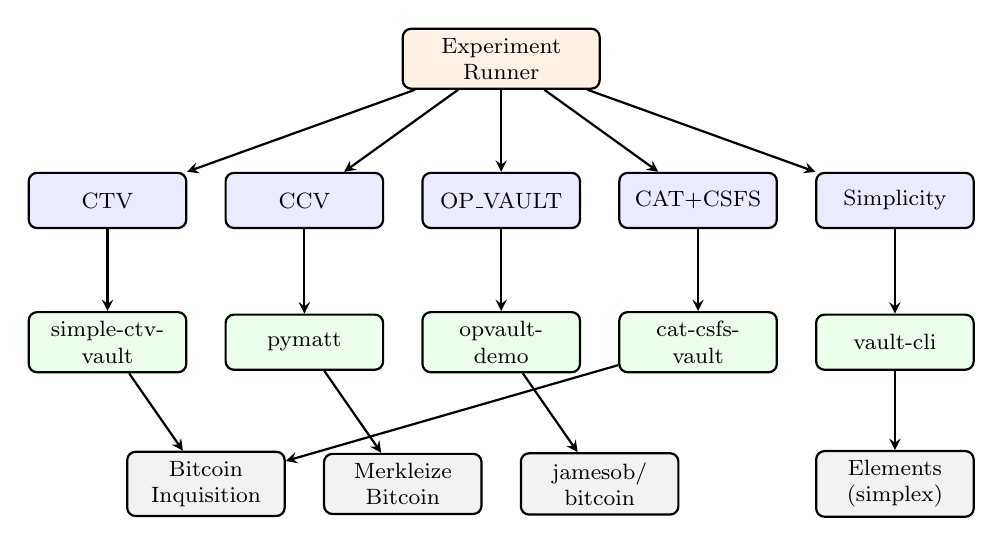
\begin{tikzpicture}[
  box/.style={rectangle, draw, rounded corners=3pt, minimum width=2cm,
              minimum height=0.7cm, font=\footnotesize, align=center},
  adapter/.style={box, fill=blue!8},
  node_box/.style={box, fill=gray!10},
  repo/.style={box, fill=green!8},
  >=stealth, thick,
]
  % Runner centered at top
  \node[box, minimum width=2.5cm, fill=orange!10] (runner) {Experiment\\Runner};

  % Adapters row — use explicit coordinates for even spacing
  \node[adapter] at (-5, -1.8) (ctv) {CTV};
  \node[adapter] at (-2.5, -1.8) (ccv) {CCV};
  \node[adapter] at (0, -1.8) (opv) {OP\_VAULT};
  \node[adapter] at (2.5, -1.8) (cat) {CAT+CSFS};
  \node[adapter] at (5, -1.8) (sim) {Simplicity};

  % Repos row
  \node[repo] at (-5, -3.6) (ctv_repo) {simple-ctv-\\vault};
  \node[repo] at (-2.5, -3.6) (ccv_repo) {pymatt};
  \node[repo] at (0, -3.6) (opv_repo) {opvault-\\demo};
  \node[repo] at (2.5, -3.6) (cat_repo) {cat-csfs-\\vault};
  \node[repo] at (5, -3.6) (sim_repo) {vault-cli};

  % Nodes row — 4 nodes, properly spaced
  % Inquisition centered between CTV and CAT positions
  \node[node_box] at (-3.75, -5.4) (inq) {Bitcoin\\Inquisition};
  \node[node_box] at (-1.25, -5.4) (merk) {Merkleize\\Bitcoin};
  \node[node_box] at (1.25, -5.4) (jamesob) {jamesob/\\bitcoin};
  \node[node_box] at (5, -5.4) (elements) {Elements\\(simplex)};

  % Arrows: runner to adapters
  \foreach \a in {ctv, ccv, opv, cat, sim}
    \draw[->] (runner) -- (\a);

  % Arrows: adapters to repos
  \foreach \a/\r in {ctv/ctv_repo, ccv/ccv_repo, opv/opv_repo, cat/cat_repo, sim/sim_repo}
    \draw[->] (\a) -- (\r);

  % Arrows: repos to nodes
  \draw[->] (ctv_repo) -- (inq);
  \draw[->] (cat_repo) -- (inq);
  \draw[->] (ccv_repo) -- (merk);
  \draw[->] (opv_repo) -- (jamesob);
  \draw[->] (sim_repo) -- (elements);
\end{tikzpicture}%
}
\caption{Framework architecture. The experiment runner invokes vault operations
through the \texttt{VaultAdapter} interface. Each adapter wraps a covenant-specific
implementation and communicates with its required Bitcoin or Elements node variant.
CTV and CAT+CSFS share the Bitcoin Inquisition node.}
\label{fig:architecture}
\end{figure}

\subsection{Adapter Interface} \label{ss:adapter_interface}

The abstract \texttt{VaultAdapter} class defines the contract that every adapter
must implement. The core lifecycle methods mirror the four-phase vault model from
Section~\ref{se:vault_lifecycle}:

\begin{itemize}
\item \texttt{create\_vault(amount\_sats)} $\rightarrow$ \texttt{VaultState}:
  Fund a new vault with the specified amount.
\item \texttt{trigger\_unvault(vault)} $\rightarrow$ \texttt{UnvaultState}:
  Initiate a withdrawal using the hot key.
\item \texttt{complete\_withdrawal(unvault)} $\rightarrow$ \texttt{TxRecord}:
  Finalize the withdrawal after the CSV delay.
\item \texttt{recover(state)} $\rightarrow$ \texttt{TxRecord}:
  Execute emergency recovery from either the Funded or Triggered state.
\end{itemize}

Optional methods expose capabilities that not all covenants support:
\texttt{trigger\_revault} for partial withdrawals (CCV, OP\_VAULT),
\texttt{trigger\_batched} for combining multiple vault UTXOs in one transaction
(CCV, OP\_VAULT), and \texttt{supports\_keyless\_recovery} for CCV's signature-free
recovery path.

\subsection{Capability-Based Dispatch} \label{ss:capability_dispatch}

Experiments query adapter capabilities at runtime rather than checking adapter names.
For example, the multi-input batching experiment calls
\texttt{adapter.supports\_batched\_trigger()} to determine whether to execute the
batched or linear code path. This design principle---dispatch on capabilities, not
identities---means a new adapter automatically participates in all experiments whose
required capabilities it declares. Table~\ref{tab:capabilities} shows the capability
matrix for the five adapters.

\begin{table}[t]
\centering
\caption{Adapter capability matrix. Experiments dispatch on these capabilities
rather than adapter names.}
\label{tab:capabilities}
\small
\begin{tabular}{@{}lccccc@{}}
\toprule
Capability & CTV & CCV & OPV & CAT & SIM \\
\midrule
\texttt{create\_vault}          & \checkmark & \checkmark & \checkmark & \checkmark & \checkmark \\
\texttt{trigger\_unvault}       & \checkmark & \checkmark & \checkmark & \checkmark & \checkmark \\
\texttt{complete\_withdrawal}   & \checkmark & \checkmark & \checkmark & \checkmark & \checkmark \\
\texttt{recover}                & \checkmark & \checkmark & \checkmark & \checkmark & \checkmark \\
\texttt{supports\_revault}      & ---        & \checkmark & \checkmark & ---        & ---        \\
\texttt{supports\_batched\_trigger} & ---    & \checkmark & \checkmark & ---        & ---        \\
\texttt{supports\_keyless\_recovery} & ---   & \checkmark & ---        & ---        & ---        \\
Address reuse safe              & No         & Yes        & Yes        & Yes        & Yes        \\
\bottomrule
\end{tabular}
\end{table}

\subsection{Implementation Provenance} \label{ss:provenance}

Three of the five vault implementations are third-party upstream repositories used
as-is: \texttt{simple-ctv-vault} (jamesob), \texttt{pymatt} (Merkleize/Ingala), and
\texttt{opvault-demo} (jamesob). The remaining two---\texttt{cat-csfs-vault} and
\texttt{simple-simplicity-vault}---are original implementations built for this research.
This distinction matters for interpreting results: implementation bugs in upstream
repositories are not attributable to the BIP design, while bugs in our own
implementations are indistinguishable from design choices unless explicitly documented.
Section~\ref{se:impl_choices} in Chapter~\ref{ch:discussion} lists the specific design
choices we made in the two original implementations.

% ======================================================================
\section{Primary Metric: Virtual Size} \label{se:metrics}

The primary metric throughout this work is \emph{virtual size} (vsize), measured in
virtual bytes (vB). Virtual size is the segwit-discounted transaction size used by
Bitcoin Core for relay policy, fee estimation, and block weight accounting:

\begin{equation} \label{eq:vsize}
\text{vsize} = \left\lceil \frac{\text{weight}}{4} \right\rceil
\quad \text{where} \quad
\text{weight} = 3 \times \text{base\_size} + \text{total\_size}
\end{equation}

\noindent
The base size excludes witness data; the total size includes it. The factor-of-4
discount on witness data reflects the segwit design decision to incentivize
witness-heavy transaction formats (Taproot, multisig) without increasing the block
size limit for non-witness data.

Virtual size is the correct metric for cross-covenant comparison because it is
\emph{structurally deterministic}: for a given script and witness structure, vsize
is identical regardless of chain state, balance, block height, or execution
environment. The per-UTXO recovery-cost scaling experiment (Chapter~\ref{ch:results})
confirmed this empirically: across 50 trigger-and-revault splits with vault
balances ranging from 50~million to fewer than 1{,}000 satoshis, the measured vsize
range was zero for both CCV and OP\_VAULT transactions.

This determinism has a methodological consequence: single-run measurements are
exact values, not estimates. There is no variance to analyze and no confidence
interval to compute. Repeated measurements would produce identical results because
the measurement is a function of the script structure, not a stochastic process.

\subsection{Fee Projection Model} \label{ss:fee_projection}

Since regtest has no fee market, we project transaction costs into real-world fee
environments using a linear model:

\begin{equation} \label{eq:fee_projection}
\text{fee}(r) = \text{vsize} \times r
\end{equation}

\noindent
where $r$ is the fee rate in sat/vB, treated as an exogenous parameter. We evaluate
all security experiments at six historically observed fee rates: 1~sat/vB (2021 low),
10~sat/vB (2022 average), 50~sat/vB (2023 moderate), 100~sat/vB (2024 inscriptions
era), 300~sat/vB (2023 BRC-20 spike), and 500~sat/vB (stress scenario). This
produces a cost sensitivity table for each attack, showing how the rationality
condition shifts across fee environments.

The rationality condition for an attack is:

\begin{equation} \label{eq:rationality}
\text{attack\_cost}(r) < \text{vault\_value}
\end{equation}

\noindent
An attack is economically rational when its on-chain cost (transaction fees plus
locked capital) is less than the value at risk in the vault. This condition is
necessary but not sufficient: the attacker must also expect the attack to succeed,
which depends on whether the defender's watchtower can respond within the CSV window.

% ======================================================================
\section{Rationality and Scope Conventions}
\label{se:rationality_conventions}

Every attack class derived in Chapter~\ref{ch:security} is accompanied
by a standardised \emph{Rationality and Scope} block with seven
fields. The fields are defined here, once, so that Chapter~\ref{ch:security}'s
derivations do not re-introduce the schema. Appendix~D carries the full
free-text form for every class; Chapter~\ref{ch:security} references
these blocks inline.

\begin{description}
\item[(1) Attacker capability.] Keys held, capital on hand, mempool
  access, compute. Cites the Kerckhoffs assumption of
  Section~\ref{ss:kerckhoffs} by reference; does not re-state it.
\item[(2) Defender model.] Watchtower authority and policy
  (proactive vs reactive, batched vs per-UTXO), user availability,
  detection-to-action latency. Where the attack depends on a specific
  defender choice, the block names it and explains why a rational
  defender might make that choice.
\item[(3) Economic preconditions.] Fee regime, vault-value range, and
  rationality threshold under which the attack yields positive
  adversary advantage.
\item[(4) Protocol / network assumptions.] Mempool policy parameters
  (descendant limits, dust thresholds, RBF rules), relay floor,
  TRUC/BIP-431 modifiers, cluster-mempool scope-limits.
\item[(5) Scope of validity.] Axis-values under which the class
  applies; equally important, the axis-values under which it does
  \emph{not} apply.
\item[(6) Rational-attacker check.] Is execution economically rational?
  Payoff vs cost vs residual (theft, liveness denial, both, or neither).
  If the attack is only rational under external incentive (extortion,
  competition, state actor), the block says so explicitly.
\item[(7) Counter-factual mitigations.] Which single falsified
  assumption kills the attack. This field doubles as a seed for
  deployment recommendations in Chapter~\ref{ch:discussion}.
\end{description}

The template applies to attack classes (Z1--Z6) in
Chapter~\ref{ch:security} and, with ``Attack'' replaced by
``Measurement'' in field (1), to empirical-cost measurements in
Chapter~\ref{ch:results}. Every field is populated, or explicitly
marked ``N/A --- [reason]''; partial blocks are treated as an audit
failure.

\section{Regtest Validity} \label{se:regtest_validity}

All experiments run on Bitcoin Core regtest (or Elements regtest for Simplicity). This
is a deliberate methodological choice: regtest provides deterministic, reproducible
execution without external dependencies. However, it limits external validity in
four specific ways.

\paragraph{No mempool competition.} Regtest mines transactions immediately on demand.
Attacks that depend on mempool dynamics---fee pinning races, front-running via mempool
observation, recovery races against timelocks---lose their temporal dimension. On
mainnet, a recovery transaction competes against the attacker's withdrawal for
confirmation within the CSV window.

\paragraph{No relay policy pressure.} Bitcoin Core's relay policy (descendant limits
at 25 transactions / 101~kvB, RBF rules, minimum relay fee) is enforced in regtest's
mempool but never stressed by competing traffic. The fee pinning experiment constructs
a 25-descendant chain that reaches the limit, but no concurrent transactions contest
for mempool space.

\paragraph{No fee market.} Fee amounts on regtest are artifacts of coin selection, not
rational economic behavior. This is why we treat vsize as the primary metric and
project fees via Equation~\ref{eq:fee_projection} rather than measuring them directly.

\paragraph{Mining is instant.} The CSV delay (e.g., 10 blocks $\approx$ 100 minutes on
mainnet) resolves in milliseconds on regtest. Time-critical races between the attacker's
withdrawal and the defender's recovery are instantaneous rather than uncertain.

Table~\ref{tab:regtest_validity} summarizes the validity status of each measurement
category on regtest.

\begin{table}[t]
\centering
\caption{Regtest validity. Structural properties transfer to mainnet; temporal and
economic dynamics do not.}
\label{tab:regtest_validity}
\small
\begin{tabular}{@{}lcc@{}}
\toprule
Property & Valid on regtest? & Primary limitation \\
\midrule
Transaction vsize and weight        & Yes (exact)     & --- \\
Script execution semantics          & Yes (identical) & --- \\
Descendant chain limits             & Yes (enforced)  & No competing traffic \\
Contract state transitions          & Yes (identical) & --- \\
Cost asymmetries (trigger vs.\ recovery) & Yes (structural) & --- \\
\midrule
Absolute fee amounts                & No (artifacts)  & No fee market \\
Recovery race timing                & No              & Instant mining \\
Mempool front-running               & No              & No competing traffic \\
Fee market confirmation pressure    & No              & No congestion \\
CSV manipulation via mining power   & No              & No adversarial miners \\
\bottomrule
\end{tabular}
\end{table}

% ======================================================================
\section{Experiment Catalog} \label{se:experiment_design}

The framework includes 15 experiments organized by scope and concern.
Table~\ref{tab:experiment_catalog} lists all experiments with their scope category,
the covenants they test, and the threat model they address.

Experiments fall into five scope categories:

\begin{itemize}
\item \textbf{Comparative.} The same test runs on all covenants; findings emerge from
  the differences in outcomes (A, B, C, F, H).
\item \textbf{Capability gap.} Tests a feature that some covenants support and others
  cannot (D, E).
\item \textbf{Covenant-specific.} Measures economic costs of design tradeoffs unique
  to one covenant (K, L, O, P).
\item \textbf{Verification.} Empirically confirms that specified opcode or
  cryptographic behavior holds in the implementation (I, M, N). These are
  implementation correctness checks, not security findings.
\item \textbf{Analytical.} Fee projections and sensitivity analysis using structural
  vsize as input; no on-chain transactions produced (J).
\end{itemize}

\begin{table}[t]
\centering
\caption{Experiment catalog. Each experiment is identified by a letter (A--P, no G)
and classified by scope and concern.}
\label{tab:experiment_catalog}
\small
\begin{tabular}{@{}cllll@{}}
\toprule
ID & Name & Category & Covenants & TM \\
\midrule
A & \texttt{lifecycle\_costs}     & Comparative   & All 5  & --- \\
B & \texttt{address\_reuse}       & Comparative   & All 5  & TM7 \\
C & \texttt{fee\_pinning}         & Comparative   & All 5  & TM1 \\
D & \texttt{revault\_amplification} & Capability gap & CCV, OPV & --- \\
E & \texttt{multi\_input}         & Capability gap & All 5  & --- \\
F & \texttt{recovery\_griefing}   & Comparative   & All 5  & TM2 \\
H & \texttt{watchtower\_exhaustion} & Comparative & CCV, OPV & TM4 \\
I & \texttt{ccv\_mode\_bypass}    & Verification  & CCV    & TM8 \\
J & \texttt{fee\_sensitivity}     & Analytical    & All    & All \\
K & \texttt{opvault\_recovery\_auth} & Covenant-specific & OPV & TM2 \\
L & \texttt{opvault\_trigger\_key\_theft} & Covenant-specific & OPV & TM3,5 \\
M & \texttt{cat\_csfs\_hot\_key\_theft} & Verification & CAT & TM9 \\
N & \texttt{cat\_csfs\_witness\_manip.} & Verification & CAT & TM10 \\
O & \texttt{cat\_csfs\_dest\_lock} & Covenant-specific & CAT & --- \\
P & \texttt{cat\_csfs\_cold\_key\_recovery} & Covenant-specific & CAT & TM11 \\
\bottomrule
\end{tabular}
\end{table}

% ======================================================================
\section{Node Infrastructure} \label{se:node_infrastructure}

Each covenant requires a specific Bitcoin (or Elements) node variant, because the
opcodes are not yet activated on Bitcoin mainnet. CTV and CAT+CSFS share Bitcoin
Inquisition, a soft-fork testing fork maintained by the Bitcoin Inquisition project.
CCV requires a separate fork maintained by Merkleize (Ingala). OP\_VAULT requires
jamesob's fork with the \texttt{2023-02-opvault-inq} branch, which uses the older
autotools build system. Simplicity runs on Elements via the Simplex toolchain, which
bundles \texttt{elementsd} and an Esplora block indexer.

\begin{table}[t]
\centering
\caption{Node variants required for each covenant. Switching nodes wipes regtest
state; experiments are isolated per-covenant.}
\label{tab:nodes}
\small
\begin{tabular}{@{}llll@{}}
\toprule
Covenant & Node variant & Branch & Build \\
\midrule
CTV       & Bitcoin Inquisition       & \texttt{v29.2-inq} release    & Pre-built \\
CCV       & Merkleize Bitcoin         & \texttt{inq-ccv}              & CMake \\
OP\_VAULT & jamesob/bitcoin           & \texttt{2023-02-opvault-inq}  & Autotools \\
CAT+CSFS  & Bitcoin Inquisition       & \texttt{v29.2-inq} release    & Pre-built \\
Simplicity & Elements (Simplex SDK)   & \texttt{v0.0.2}               & Pre-built \\
\bottomrule
\end{tabular}
\end{table}

The framework's \texttt{switch-node.sh} script manages node lifecycle: starting the
correct node variant, wiping regtest state between runs, and discovering ports for
Elements (which assigns random RPC and Esplora ports at startup). A Docker image
packages all five node variants with pre-built binaries for reproducible execution
without local compilation.
